\section{Task 1: attacks on the intrusion detector}

\lead{Outcome.} Membership inference failed: 0.535 against a 50\% guess, below a blind control. Evasion worked on Wednesday's data. A black-box attacker cut detection to 0.350 at a change cap of $\vtheta=0.25$, and to 0.000 at 0.5. The changes are seconds of timing: real, but not subtle. A 300-flow Thursday sample agrees (below).

\lead{Target.} We attack the \emph{first version} of the Lab~1 model, a small neural network (a rescaling step, then two hidden layers of 64 and 32 units). Our reproduction matches its metrics to six decimals.
\begin{itemize}
\item \textbf{Data:} CICIDS-2018 network flows from Wednesday 14 February 2018, Benign against Attack, 77 features.
\item \textbf{Split:} 70/30 by row order: 731{,}322 training and 313{,}424 test rows. The rows are sorted by the raw timestamp, which uses a 12-hour clock without AM/PM, so this is \emph{not} true time order. 377{,}414 training rows (the 13:00--17:30 afternoon) come after the 11:03--12:59 test window, and FTP brute force appears in both parts. Clean accuracy is therefore optimistic.
\item \textbf{Access:} the black-box attacks used only its HTTP scoring API. The API returns the attack score, the label at the 0.5 threshold, and the logit margin. PGD-40 and 1C used the weights.
\end{itemize}

\lead{Why not the submitted Lab~1 model.} The submitted Lab~1 repairs the clock, drops the 10 constant columns (67 features) and trains a 128--64 network. Its Wednesday test window then holds only SSH brute force, which training never saw, and it flags 30 of 187{,}589 attack flows (recall 0.0002): there is nothing left for evasion to remove. Lab~1 itself reports our split as its unrepaired-clock control. Our results describe the first-version model, not the submitted one.

\lead{Threat model of each attack.}
\begin{itemize}
\item \textbf{1A membership inference:} black box, one query per flow. Needs each flow's true label and a labelled calibration pool.
\item \textbf{1B random search and FD-FGSM:} black box, score queries only. Needs the feature schema and the mutable features.
\item \textbf{1B PGD-40:} white box, uses the weights. It is not always the strongest attack. On the two-round model FD-FGSM did better at $\vtheta=0.15$ (detection 0.000 against 0.350, see 1C).
\end{itemize}

\subsection{1A --- Membership inference: a negative result}

We thresholded confidence, loss and logit margin, fitting thresholds on a disjoint calibration pool (20{,}000 members and non-members per day).

\lead{Membership-inference accuracy against the 50\% guess.}
\begin{center}\small
\begin{tabular}{@{}llccc@{}}
\toprule
\textbf{Day} & \textbf{Attack} & \textbf{Accuracy} & \textbf{95\% CI} & \textbf{Blind control (no queries)} \\
\midrule
Wednesday & confidence / margin / loss & 0.5352 & [0.5303, 0.5401] & \textbf{0.5472} \\
Thursday  & confidence / margin / loss & 0.5280 & [0.5230, 0.5329] & \textbf{0.5703} \\
Wednesday, two-round model & confidence / margin & 0.5349 & [0.5300, 0.5398] & \textbf{0.5472} \\
\bottomrule
\end{tabular}
\end{center}

\lead{Why it fails.} The textbook expects membership inference to beat chance only as far as the model memorised its training rows. We measured 0.535: above the 50\% guess but \emph{below} the blind control, which never queries the model. The signal is distribution shift across the train/test split (attack share 33.87\% in Wednesday training, 42.51\% in test), not a leak. The train/test gap is near zero ($+4\times10^{-6}$ Wednesday, $-0.0026$ Thursday), and 56.5\% of Wednesday and 36.9\% of Thursday test rows duplicate a training row exactly. The two-round model behaves the same (third row). \textbf{Finding F6: not exploitable as deployed.}

\subsection{1B --- Evasion: detection rate against change size}

Evasion asks: how much must an attacker change an attack flow before the detector calls it benign? (Methods: Key terms.)

\lead{Which features an attacker can change.} \textbf{52 of 77 features are mutable} (own packet sizes, pacing, flag counts, forward counters) and \textbf{25 are not} (server replies, victim-derived ratios, both-direction aggregates). A projection keeps changes physically consistent, for example non-negative durations. The limit $\vtheta$ (Key terms) caps each feature separately, so the allowed changes form a box around the original flow.

\lead{Detection rate against change size.} Wednesday uses 300 attack flows the model already scores above 0.9. The last three columns repeat the three attacks on a Thursday sample (see below). Cost per 300 flows: 60{,}300 queries for random search, 31{,}200 for FD-FGSM, 12{,}000 gradients for PGD.

\lead{Thursday: a 300-flow sample, not the whole day.} Evasion also works on a second day, but this sample cannot say how often. We repeated 1B on the Thursday model. Only 1{,}559 of 35{,}338 Thursday attack test flows score above 0.9. We kept those and drew 300 with seed 42, so the sample holds the attacks the model is most sure of. At $\vtheta=0.25$ the detector still caught 296/300 under random search, but only 29/300 under FD-FGSM and 91/300 under PGD-40.

\begin{center}\small
\begin{tabular}{@{}lccc@{\hskip 10pt}ccc@{}}
\toprule
& \multicolumn{3}{c}{\textbf{Wednesday}} & \multicolumn{3}{c}{\textbf{Thursday sample}} \\
\cmidrule(r){2-4}\cmidrule(l){5-7}
$\vtheta$ & random & FD-FGSM & PGD-40 & random & FD-FGSM & PGD-40 \\
\midrule
0.010 & 1.000 & 1.000 & 1.000 & 1.000 & 1.000 & 1.000 \\
0.025 & 1.000 & 1.000 & 1.000 & 1.000 & 1.000 & 1.000 \\
0.050 & 1.000 & 1.000 & 1.000 & 1.000 & 1.000 & 1.000 \\
0.100 & 1.000 & 0.973 & 0.973 & 1.000 & 1.000 & 1.000 \\
0.150 & 1.000 & 0.897 & 0.897 & 1.000 & 0.510 & 0.970 \\
0.250 & 0.973 & 0.350 & 0.350 & 0.987 & \textbf{0.097} & \textbf{0.303} \\
0.500 & 0.743 & \textbf{0.000} & \textbf{0.000} & 0.197 & 0.040 & 0.070 \\
\bottomrule
\end{tabular}
\end{center}

\lead{Benign pushed toward attack (alert flooding, framing).} We reversed the attack on 300 Wednesday benign flows (0/300 false alarms before the attack). Up to $\vtheta=0.25$ at most 4/300 became false alarms, for any method. At $\vtheta=0.5$, 85/300 did (FD-FGSM). Flooding analysts needs much larger changes than evasion.

\begin{figure}[htbp]\centering
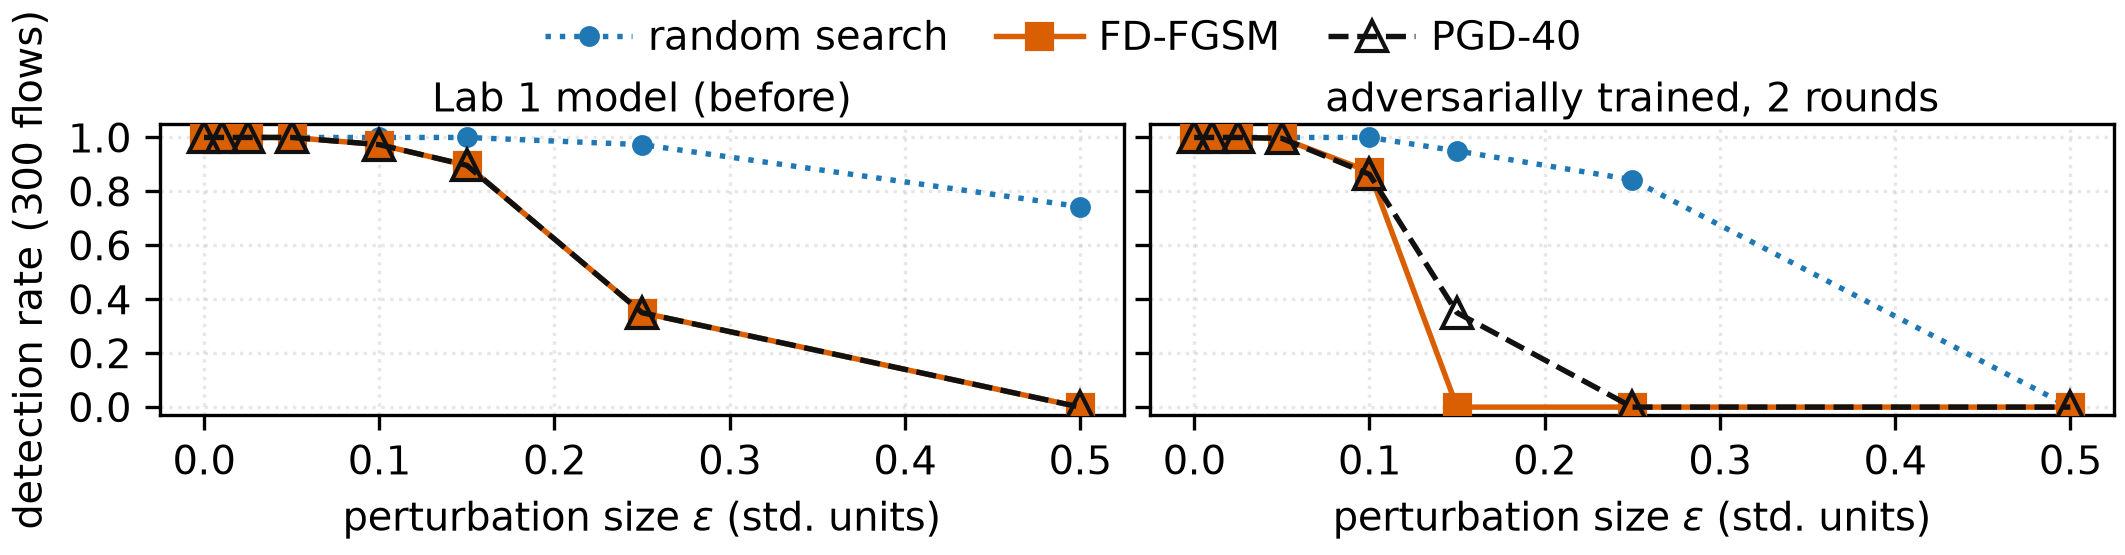
\includegraphics[width=0.62\textwidth]{task1b_evasion.png}
\caption{Detection rate against perturbation size ($n=300$ flows per point). Left: the Lab~1 model; FD-FGSM and PGD-40 coincide (PGD dashed). Right: after adversarial training (1C).}\label{fig:curves}
\end{figure}

\lead{What the curves show} (Fig.~\ref{fig:curves}, left). The ordering is the result. Random search barely dents the detector (0.743 at $\vtheta=0.5$), while one finite-difference gradient evades completely. A random-search-only test would call it robust. The textbook expects PGD-40 to beat a single-step attack; here FD-FGSM matched it at every $\vtheta$. We did not test why.

\lead{Realism in traffic units.} At $\vtheta=0.25$ successful changes move 44 of 52 mutable features. They shift \texttt{Fwd IAT Tot} (total time between forward packets) by $+6.7$\,s and \texttt{Flow IAT Max} (longest gap between two packets) by $+3.5$\,s. At $\vtheta=0.10$, where evasion first appears, they still move 2.7\,s and 1.4\,s: seconds, not milliseconds. In our judgement (not measured), a rule or a human would notice, so this is not realistic for a careful attacker. \textbf{Finding F5.}

\lead{What a real attacker would need to know.} Score access to the API (its label and margin leak more); no weights. The feature schema and which 52 features they control. The per-feature scale (standard deviation $\sigma_j$), to size a change. A budget of 104 queries per flow for FD-FGSM and up to 201 for random search; a rate limit only delays this. For 1A, true labels and a calibration pool. Scoring one flow takes a median 0.12\,ms, so probing speed is set by the network and any rate limit (\S5).

